\documentclass[12pt]{article}

\usepackage{fullpage}
\usepackage{amsfonts}
\usepackage{graphicx}
\usepackage{hyperref}
\usepackage{standalone}
\usepackage{amsmath}
\usepackage[margin=1.0in, paperwidth=8.5in]{geometry}
\usepackage{dsfont}
\usepackage{wrapfig}
\usepackage{cite}
\usepackage{relsize}
\usepackage{amssymb}
\usepackage[shortlabels]{enumitem}
\usepackage{IEEEtrantools}
\usepackage{authblk}
\usepackage{setspace}

\begin{document}

\title{Numerical Notes}
\author{}
\date{\today}

\maketitle


\section{Number of modes, N}
Let $L$ be the length of our domain, $\kappa$ be the coefficient of molecular diffusion, $U$ be the RMS velocity for the energy-constrained case, and $\gamma$ be the RMS rate-of-strain for the enstrophy-constrained case. We know that the Batchelor scale is given by 
\begin{equation}
l=\kappa/ U
\end{equation}
for the energy-constrained case or 
\begin{equation}
l=\sqrt{\kappa/\gamma}.
\end{equation}
So we would like the maximum wavenumber to be $k_{max}=(2\pi /L) (N/2) >2\pi/l$. We get the following criteria,
\begin{equation}
N > 2L/l.
\end{equation}
This becomes
\begin{equation}
N > 2L U/\kappa
\end{equation}
for the energy-constrained case or
\begin{equation}
N > 2L \sqrt{\gamma/ \kappa}
\end{equation}
for the enstrophy-constrained case.

\subsection{Boyd's rule-of-thumb}
Estimate the number of wavelengths,$M =L/l$ where $l$ is the smallest scaled needed to be resolved. Then, use the following formula (justified in Boyd, Pg 55)
\begin{equation}
N\geq6+4(M-1)
\end{equation}
So, for the energy case, we have
\begin{equation}
N\geq 6+4\left(\frac{LU}{\kappa}-1\right),
\end{equation}
and for the enstrophy case, we have
\begin{equation}
N\geq 6+4\left(L\sqrt{\frac{\gamma}{\kappa}}-1\right).
\end{equation}



\section{CFL condtion}

Using the CFL condition,
\begin{equation}
h < \frac{ \Delta x}{u} .
\end{equation}
$\Delta x$ is the resolved smallest scale; $\Delta x=\frac{2\pi}{k_{max}} = 2L/N$. $u$ is the velocity scale. For the energy-constrained case, this is simply $u=U$. For the enstrophy-constrained case, this is simply $u=\gamma L$. This condition becomes
\begin{equation}
h < \frac{2L }{U N} 
\end{equation}
for the energy-constrained case or
\begin{equation}
h < \frac{2}{\gamma N} 
\end{equation}
for the enstrophy-constrained case. The above criteria will be used for fixed time-stepping. We will implement RKF45 with adaptive timestepping so that we can have more robust code and maintain stability throughout simulation.

\section{Numerical time integration}

Given that our domain is doubly periodic, a natural basis is the set of Fourier functions. We evolve the advection equation in Fourier space. This is given by

\begin{equation}
\label{eq:original_DE}
\frac{d}{d t} \hat{\theta}_{\mathbf{k}} = \mathcal{F}_{\mathbf{k}}(- \mathbf{u}\cdot\nabla \theta) - \kappa |\mathbf{k}|^{2}\hat{\theta}_{\mathbf{k}}
\end{equation}
for each mode $\mathbf{k}$. 
\subsection{Method 1: Forward Euler without integration factor}

\subsection{Method 2: Forward Euler with integration factor}

\subsection{Method 3: Cash-Karp adaptive time-stepping method without integration factor}

\subsection{Method 4: Cash-Karp adaptive time-stepping method with integration factor }

We will first perform an operator splitting procedure. By introducing the following change of variables, we have 
\begin{equation}
\label{eq:change_of_variables}
\hat{\phi}_{\mathbf{k}}(t)= \hat{\theta}_{\mathbf{k}}(t)e^{\kappa |\mathbf{k}|^{2}t}
\end{equation}
We find that 
\begin{equation}
\frac{d}{dt}(\hat{\phi}_{\mathbf{k}})e^{-\kappa |\mathbf{k}|^{2}t} -\kappa |\mathbf{k}|^{2} \hat{\phi}_{\mathbf{k}}e^{-\kappa |\mathbf{k}|^{2}t} = \mathcal{F}_{\mathbf{k}}(- \mathbf{u}\cdot\nabla \theta) - \kappa |\mathbf{k}|^{2}\hat{\phi}_{\mathbf{k}}e^{-\kappa |\mathbf{k}|^{2}t}
\end{equation} 
which simplifies to 
\begin{equation}
\frac{d}{dt}(\hat{\phi}_{\mathbf{k}})= e^{\kappa |\mathbf{k}|^{2}t}\mathcal{F}_{\mathbf{k}}(- \mathbf{u}\cdot\nabla \theta)  = e^{\kappa |\mathbf{k}|^{2}t}\hat{\Theta}_{\mathbf{k}}(\hat{\theta}_{\mathbf{k}'}) =\hat{\Phi}_{\mathbf{k}}(t,\hat{\phi}_{\mathbf{k}'}) 
\end{equation} 
where 
\begin{equation}
\Theta_{\mathbf{k}}(\hat{\theta}_{\mathbf{k}'})=\mathcal{F}_{\mathbf{k}}(- \mathbf{u}(\hat{\theta}_{\mathbf{k}'})\cdot\nabla \mathcal{F}^{-1}(\hat{\theta}_{\mathbf{k}'}))
\end{equation}
and
\begin{multline}
\Phi_{\mathbf{k}}(t,\hat{\phi}_{\mathbf{k}'})=e^{\kappa |\mathbf{k}|^{2}t}\Theta_{\mathbf{k}}(\hat{\theta}_{\mathbf{k}'}=\hat{\phi}_{\mathbf{k}'}(t)e^{-\kappa |\mathbf{k}'|^{2}t})\\
=e^{\kappa |\mathbf{k}|^{2}t}\mathcal{F}_{\mathbf{k}}(- \mathbf{u}(\hat{\theta}_{\mathbf{k}'}=\hat{\phi}_{\mathbf{k}'}(t)e^{-\kappa |\mathbf{k}'|^{2}t})\cdot\nabla \mathcal{F}^{-1}(\hat{\theta}_{\mathbf{k}'}=\hat{\phi}_{\mathbf{k}'}(t)e^{-\kappa |\mathbf{k}'|^{2}t}))
\end{multline}
In a sense we have `exactly solved' the linear part of (\ref{eq:original_DE}) (If $\mathbf{u}$ is identically zero throughout the domain, then (\ref{eq:change_of_variables}) is exact with $\hat{\phi}_{\mathbf{k}}(t)=\hat{\theta}_{\mathbf{k}}(0)$).    

Now, we implement our time-stepping scheme. We use the embedded Runge-Kutta-Fehlberg 4(5) (RKF45) method with Cash-Karp Parameters.  The associated fifth-order formula is given by 
\begin{equation}
\hat{\phi}_{\mathbf{k}}^{j+1}=\hat{\phi}_{\mathbf{k}}^{j}+c_{1}\hat{g}_{\mathbf{k},1}  + c_{2}\hat{g}_{\mathbf{k},2} + \dots +  c_{6}\hat{g}_{\mathbf{k},6}  + O(h^{6})
\end{equation}
while the embedded fourth-order formula is 
\begin{equation}
\hat{\phi}_{\mathbf{k}}^{j+1 , *}=\hat{\phi}_{\mathbf{k}}^{j, *}+c_{1}^{*}\hat{g}_{\mathbf{k},1}  + c_{2}^{*}\hat{g}_{\mathbf{k},2} + \dots +  c_{6}^{*}\hat{g}_{\mathbf{k},6} + O(h^{5}).
\end{equation}
where 
\begin{subequations}
	\begin{align}
		\hat{g}_{\mathbf{k},1} & = h \hat{\Phi}_{\mathbf{k}}(t^{j} \, , \, \hat{\phi}^{j}_{\mathbf{k}}) \\
		\hat{g}_{\mathbf{k},2} & = h \hat{\Phi}_{\mathbf{k}}(t^{j}+a_{2}h \, , \, \hat{\phi}^{j}_{\mathbf{k}} + b_{21}\hat{g}_{\mathbf{k},1}  ) \\
		\notag
		\vdots \\
		\hat{g}_{\mathbf{k},6} & = h \hat{\Phi}_{\mathbf{k}}(t^{j}+a_{6}h \, , \, \hat{\phi}^{j}_{\mathbf{k}} + b_{61}\hat{g}_{\mathbf{k},1}  + \dots +    b_{65}\hat{g}_{\mathbf{k},5} ) .
	\end{align}
\end{subequations}


Substituting in $\hat{\theta}$, the fifth-order formula becomes
\begin{equation}
e^{\kappa |\mathbf{k}|^{2}(t^{j}+h)}\hat{\theta}_{\mathbf{k}}^{j+1}=e^{\kappa |\mathbf{k}|^{2}(t^{j})}\hat{\theta}_{\mathbf{k}}^{j}+ c_{1}\hat{g}_{\mathbf{k},1}  + c_{2}\hat{g}_{\mathbf{k},2} + \dots +  c_{6}\hat{g}_{\mathbf{k},6}  + O(h^{6})
\end{equation}
and the embedded fourth-order formula is
\begin{equation}
e^{\kappa |\mathbf{k}|^{2}(t^{j}+h)}\hat{\theta}_{\mathbf{k}}^{j+1,*}=e^{\kappa |\mathbf{k}|^{2}(t^{j})}\hat{\theta}_{\mathbf{k}}^{j}+ c_{1}^{*}\hat{g}_{\mathbf{k},1}  + c_{2}^{*}\hat{g}_{\mathbf{k},2} + \dots +  c_{6}^{*}\hat{g}_{\mathbf{k},6}  + O(h^{6})
\end{equation}
where
\begin{subequations}
	\begin{align}
		\hat{g}_{\mathbf{k},1} & = h e^{\kappa |\mathbf{k}|^{2}(t^{j})}\hat{\Theta}_{\mathbf{k}}(\hat{\theta}_{\mathbf{k}'}=(\hat{\theta}_{\mathbf{k}'}^{j}e^{\kappa |\mathbf{k}'|^{2}t^{j}})e^{-\kappa |\mathbf{k}'|^{2}t^{j}}) \\
		\hat{g}_{\mathbf{k},2} & = h e^{\kappa |\mathbf{k}|^{2}(t^{j}+a_{2}h)}\hat{\Theta}_{\mathbf{k}}(\hat{\theta}_{\mathbf{k}'}=((\hat{\theta}_{\mathbf{k}'}^{j}e^{\kappa |\mathbf{k}'|^{2}t^{j}}) + b_{21}\hat{g}_{\mathbf{k},1}  ) e^{-\kappa |\mathbf{k}'|^{2}(t^{j}+a_{2}h)})\\
		\notag
		\vdots \\
		\hat{g}_{\mathbf{k},6} & = h e^{\kappa |\mathbf{k}|^{2}(t^{j}+a_{6}h)}\hat{\Theta}_{\mathbf{k}}(\hat{\theta}_{\mathbf{k}'}=((\hat{\theta}_{\mathbf{k}'}^{j}e^{\kappa |\mathbf{k}'|^{2}t^{j}})+ b_{61}\hat{g}_{\mathbf{k},1}  + \dots +    b_{65}\hat{g}_{\mathbf{k},5} ) e^{-\kappa |\mathbf{k}'|^{2}(t^{j}+a_{6}h)})
	\end{align}
\end{subequations}
Finally by introducing $\hat{s}_{\mathbf{k},n}=e^{-\kappa |\mathbf{k}|^{2}t^{j}}\hat{g}_{\mathbf{k},n}$, we can eliminate our dependence on the total time $t^j$.  The fifth-order formula becomes
\begin{equation}
\label{eq:fifthorder}
\hat{\theta}_{\mathbf{k}}^{j+1}=e^{-\kappa |\mathbf{k}|^{2}h}(\hat{\theta}_{\mathbf{k}}^{j}+ c_{1}\hat{s}_{\mathbf{k},1}  + c_{2}\hat{s}_{\mathbf{k},2} + \dots +  c_{6}\hat{s}_{\mathbf{k},6})  + O(h^{6})
\end{equation}
and the embedded fourth-order formula is
\begin{equation}
\label{eq:fourthorder}
\hat{\theta}_{\mathbf{k}}^{j+1,*}=e^{-\kappa |\mathbf{k}|^{2}h}(\hat{\theta}_{\mathbf{k}}^{j}+  c_{1}^{*}\hat{s}_{\mathbf{k},1}  + c_{2}^{*}\hat{s}_{\mathbf{k},2} + \dots +  c_{6}^{*}\hat{s}_{\mathbf{k},6})  + O(h^{6})
\end{equation}
where
\begin{subequations}
	\begin{align}
		\hat{s}_{\mathbf{k},1} & = h \hat{\Theta}_{\mathbf{k}}(\hat{\theta}_{\mathbf{k}'}=\hat{\theta}_{\mathbf{k}'}^{j}) \\
		\hat{s}_{\mathbf{k},2} & = h e^{\kappa |\mathbf{k}|^{2}a_{2}h}\hat{\Theta}_{\mathbf{k}}(\hat{\theta}_{\mathbf{k}'}=e^{-\kappa |\mathbf{k}'|^{2}a_{2}h}(\hat{\theta}_{\mathbf{k}'}^{j} + b_{21}\hat{s}_{\mathbf{k},1} ) )\\
		\notag
		\vdots \\
		\hat{s}_{\mathbf{k},6} & = h e^{\kappa |\mathbf{k}|^{2}a_{6}h}\hat{\Theta}_{\mathbf{k}}(\hat{\theta}_{\mathbf{k}'}=e^{-\kappa |\mathbf{k}'|^{2}a_{6}h}(\hat{\theta}_{\mathbf{k}'}^{j} + b_{61}\hat{s}_{\mathbf{k},1}+ b_{61}\hat{s}_{\mathbf{k},1} + \dots + b_{65}\hat{s}_{\mathbf{k},5} ) )
	\end{align}
\end{subequations}



The error estimate is given by the magnitude of the complex difference between (\ref{eq:fifthorder}) and (\ref{eq:fourthorder}),

\begin{equation}
\epsilon_{\mathbf{k}}\equiv |\hat{\theta}_{\mathbf{k}}^{j+1}-\hat{\theta}_{\mathbf{k}}^{j+1,*}| = \left|\sum_{i=1}^{6} (c_{i}-c_{i}^{*})\hat{s}_{\mathbf{k},i} e^{-\kappa |\mathbf{k}|^{2}h}\right| 
\end{equation}
\begin{figure*}
	\centering
	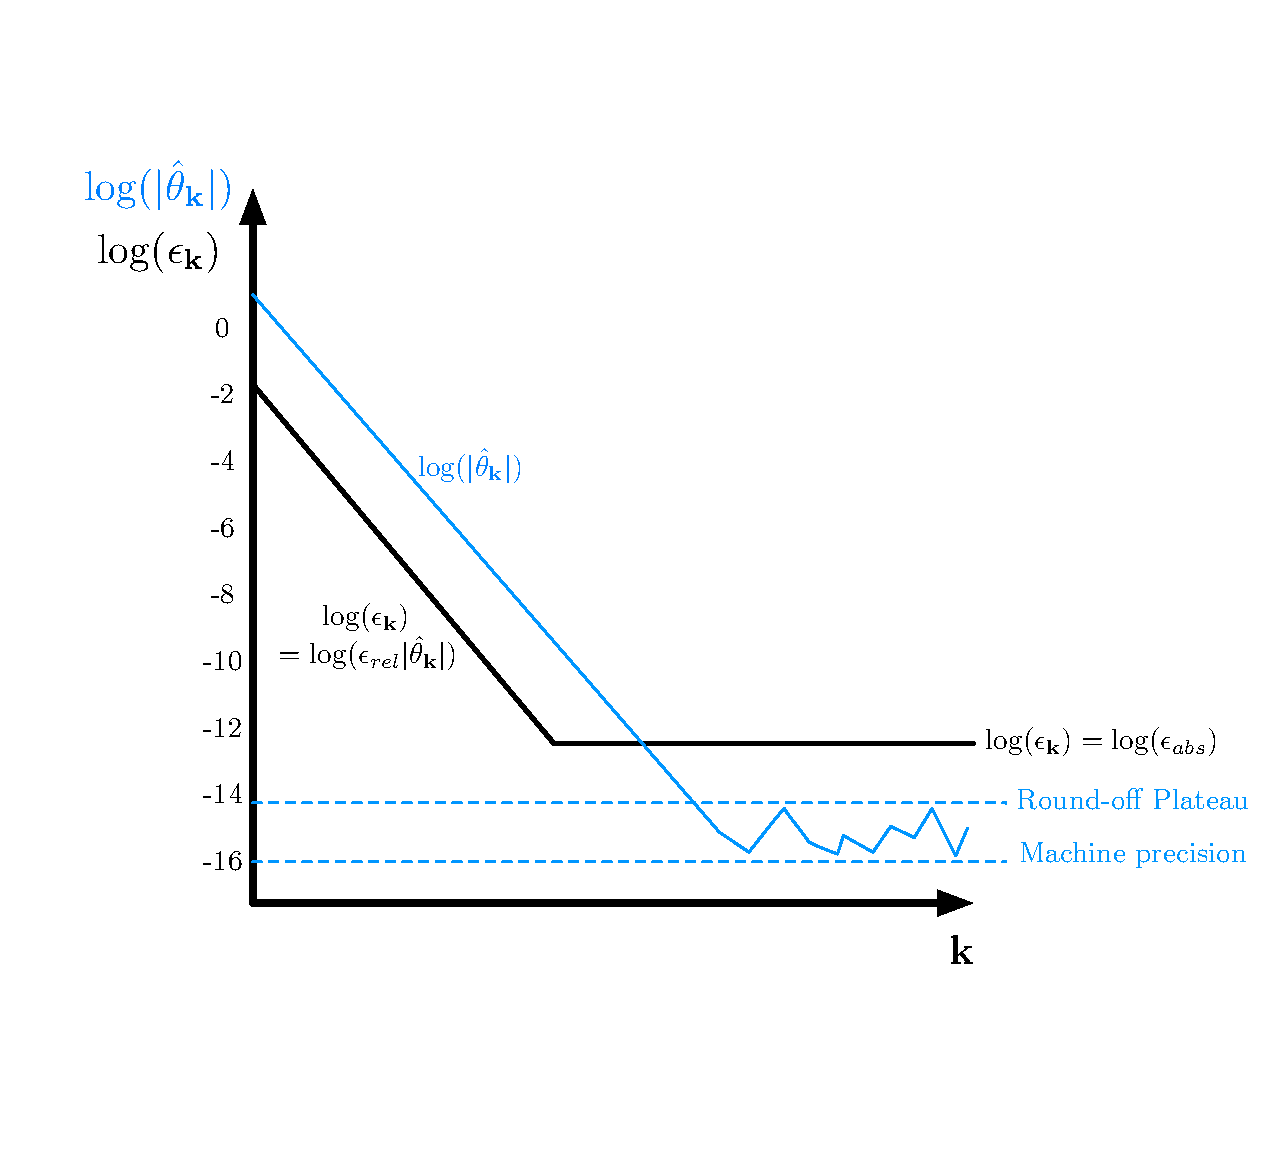
\includegraphics[width=0.6\textwidth]{spectrum_errors.eps}
	\caption{Error analysis.}
	\label{fig:spectrum_errors}
\end{figure*}

We will accept a solution if 
\begin{equation}
\label{eq:acceptance_criteria}
\epsilon_{\mathbf{k}}< \epsilon_{\mathbf{k},d} =  \max(\epsilon_{rel}|\hat{\theta}_{\mathbf{k}}|, \epsilon_{abs})
\end{equation}
for all $\mathbf{k}$. For instance, we may choose $\epsilon_{rel}=10^{-6}$ and $\epsilon_{abs}=10^{-9}$. Ideally, we would demand that $\epsilon_{\mathbf{k}}< \epsilon_{rel}|\hat{\theta}_{\mathbf{k}}|$ for all $\mathbf{k}$. This is , however, not possible since $|\hat{\theta}_{\mathbf{k}}| \gtrsim \epsilon_{m} \approx 2.22 \times 10^{-16} $ due to machine round-off error. Therefore demanding that  $\epsilon_{\mathbf{k}}< \epsilon_{rel}|\hat{\theta}_{\mathbf{k}}|$ for all $\mathbf{k}$ is unrealistic and impossible for small $|\hat{\theta}_{\mathbf{k}}| \sim \epsilon_{m}$ since $\epsilon_{\mathbf{k}} $ is also bounded from below by  $\epsilon_{m}$ due to machine round-off error. 

We then pick out the mode $\mathbf{k}^{*}$ that violates criteria (\ref{eq:acceptance_criteria}) `the most' defined by
\begin{equation}
\mathbf{k}^{*}=argmax_{\mathbf{k}} \epsilon_{\mathbf{k}}-\epsilon_{\mathbf{k},d}.
\end{equation}
Since (\ref{eq:fourthorder}) is fourth-order, we know the error estimate is approximately $\epsilon_{\mathbf{k}^{*}}=d h^{5}$ for some constant $d$. Then this gives us the constant $d= \epsilon_{\mathbf{k}^{*}}/h^5$. Thus, we can then use this to chose a new step size $h_{new}$ to achieve a desired  error $\epsilon_{d}$ by 
\begin{equation}
h_{new}=h \left(\frac{\epsilon_{\mathbf{k}^{*},d}}{\epsilon_{\mathbf{k}^{*}}}\right)^{1/5}.
\end{equation}
It is common to modify this relation by introducing a safety parameter $\beta $ that is slightly less than 1 (=0.8 or 0.9) and conditionally changing the exponent. The recommended prescription is 
\begin{eqnarray}
h := \beta h \left(\frac{\epsilon_{\mathbf{k}^{*},d}}{\epsilon_{\mathbf{k}^{*}}}\right)^{1/5} \, ,\, \epsilon \geq \epsilon_{d} \\
h := \beta h \left(\frac{\epsilon_{\mathbf{k}^{*},d}}{\epsilon_{\mathbf{k}^{*}}}\right)^{1/4}\, ,\, \epsilon <\epsilon_{d} .
\end{eqnarray}
\begin{figure*}
	\centering
	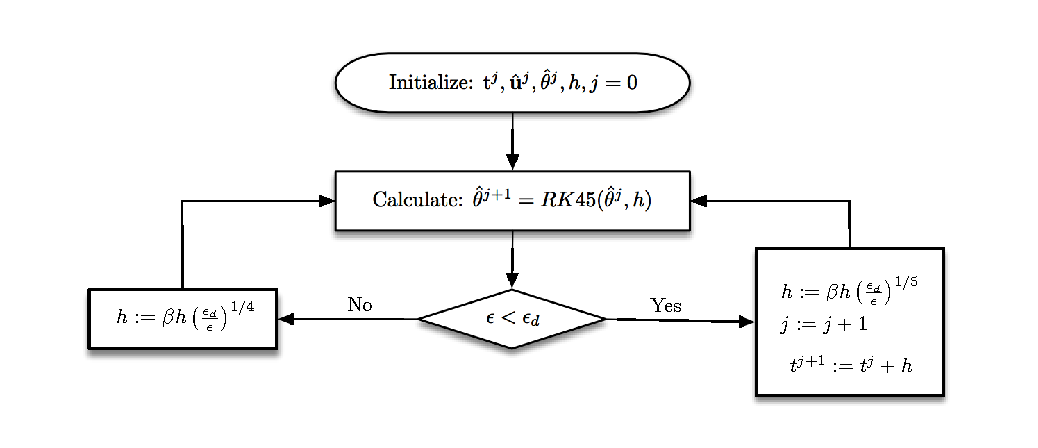
\includegraphics[width=1.0\textwidth]{RK45.eps}
	\caption{RKF45 flow diagram for adaptive time-stepping.}
	\label{fig:RKF45}
\end{figure*}
The adaptive time-stepping scheme in RKF45 is shown in figure \ref{fig:RKF45}. 

Since the step decision is based on the error scaling with $h$ of the fourth-order formula, we will use the fourth-order formula as our final update: $\hat{\theta}_{\mathbf{k}}(t^{j+1})=\hat{\theta}_{\mathbf{k}}^{j+1,*}$.

\subsection{Method 5: Semi-implicit multistep method, AB3CN [(12.33) in Boyd] }

\section{Testing}

\subsection{Derivative testing}

\subsection{Comparison to other time-stepping methods}
Methods:
\begin{enumerate}
\item  Forward Euler
\item RK4 
\item RKF45 without operator splitting
\end{enumerate}
Measured quantities:
\begin{enumerate}
\item Computation time
\item Convergence rate
\item Error
\end{enumerate}

\subsection{L2 Decay}
\subsection{Absolute stability and CFL condition}

\subsection{Spectral Blocking Problem}

Spectral block appears when the relative error $\chi$ is too large. My guess is that the method lies out of the stability region for high $\chi$ which results in high $h$. Spectral blocking is only a problem when $\kappa$ is too small. This make sense because the diffusion damps the higher modes and prevents numerical instability from amplifying over time. Note that the adaptive time stepping scheme does {\it not } control the global error. It provides an estimate of the local truncation error. So, it is possible to obtain a desired local error $\epsilon_{d}$ and not succeed at the same precision for the global error due to absolute instabilty. 

\subsection{Under-resolved issues}
The highest resolved modes in the simulation are those near the two-thirds dealiasing rule boundary. A rule-of-thumb is that the precision of a method is equal to the magnitude of these modes near the dealias boundary. We use the following quantity to flag under-resolved simulations:
\begin{equation}
\alpha = \max_{\mathbf{k}\in B_{dealis}} |\theta_{\mathbf{k}} |
\end{equation}
where $B_{dealias}=\{ \mathbf{k}=(k_{x},k_{y})  \; \; | \; \; \frac{2}{3}\left(\frac{N}{2}\right)- 1< |\mathbf{k}| <\frac{2}{3}\left(\frac{N}{2}\right)\}$. If $\alpha >\theta$ where machine precision $\epsilon_{m}=2^{-52} \approx 2.22 \times 10^{-16}$, we flag this as underresolved. 

\subsection{Case Study 1: Old and new version comparison}
(12/15/16) Results from the energy-constrained case with $N=0.5$,$dt=0.0001$, $L=2\pi$, and $\kappa$ performed on 12/3/16, differ slightly from the results from the newest version with identical numerical method (Forward-Euler). A major change has included a transition from using fftn/ifftn to rfftn/irfftn. 
\\

Results:
\begin{enumerate}
\item Found bug in functions calculateScalarH1Norm() and calculateScalarMixNorm() in new code. Fixed.
\item new code ran in 12 mins while old code ran in 43 mins. 4x speed up by using recommendations from Mortensen, 2015.
\item found bug in loading initial condition. fftn should have been rfftn
\end{enumerate}

(12/15/2016) Old and new code generate the same results now up to round-off error. Code is pushed to github and saved under "Case study 1 12/15/16" to test Folder with output results




\end{document}